\documentclass[1p]{elsarticle_modified}
%\bibliographystyle{elsarticle-num}

%\usepackage[colorlinks]{hyperref}
%\usepackage{abbrmath_seonhwa} %\Abb, \Ascr, \Acal ,\Abf, \Afrak
\usepackage{amsfonts}
\usepackage{amssymb}
\usepackage{amsmath}
\usepackage{amsthm}
\usepackage{scalefnt}
\usepackage{amsbsy}
\usepackage{kotex}
\usepackage{caption}
\usepackage{subfig}
\usepackage{color}
\usepackage{graphicx}
\usepackage{xcolor} %% white, black, red, green, blue, cyan, magenta, yellow
\usepackage{float}
\usepackage{setspace}
\usepackage{hyperref}

\usepackage{tikz}
\usetikzlibrary{arrows}

\usepackage{multirow}
\usepackage{array} % fixed length table
\usepackage{hhline}

%%%%%%%%%%%%%%%%%%%%%
\makeatletter
\renewcommand*\env@matrix[1][\arraystretch]{%
	\edef\arraystretch{#1}%
	\hskip -\arraycolsep
	\let\@ifnextchar\new@ifnextchar
	\array{*\c@MaxMatrixCols c}}
\makeatother %https://tex.stackexchange.com/questions/14071/how-can-i-increase-the-line-spacing-in-a-matrix
%%%%%%%%%%%%%%%

\usepackage[normalem]{ulem}

\newcommand{\msout}[1]{\ifmmode\text{\sout{\ensuremath{#1}}}\else\sout{#1}\fi}
%SOURCE: \msout is \stkout macro in https://tex.stackexchange.com/questions/20609/strikeout-in-math-mode

\newcommand{\cancel}[1]{
	\ifmmode
	{\color{red}\msout{#1}}
	\else
	{\color{red}\sout{#1}}
	\fi
}

\newcommand{\add}[1]{
	{\color{blue}\uwave{#1}}
}

\newcommand{\replace}[2]{
	\ifmmode
	{\color{red}\msout{#1}}{\color{blue}\uwave{#2}}
	\else
	{\color{red}\sout{#1}}{\color{blue}\uwave{#2}}
	\fi
}

\newcommand{\Sol}{\mathcal{S}} %segment
\newcommand{\D}{D} %diagram
\newcommand{\A}{\mathcal{A}} %arc


%%%%%%%%%%%%%%%%%%%%%%%%%%%%%5 test

\def\sl{\operatorname{\textup{SL}}(2,\Cbb)}
\def\psl{\operatorname{\textup{PSL}}(2,\Cbb)}
\def\quan{\mkern 1mu \triangleright \mkern 1mu}

\theoremstyle{definition}
\newtheorem{thm}{Theorem}[section]
\newtheorem{prop}[thm]{Proposition}
\newtheorem{lem}[thm]{Lemma}
\newtheorem{ques}[thm]{Question}
\newtheorem{cor}[thm]{Corollary}
\newtheorem{defn}[thm]{Definition}
\newtheorem{exam}[thm]{Example}
\newtheorem{rmk}[thm]{Remark}
\newtheorem{alg}[thm]{Algorithm}

\newcommand{\I}{\sqrt{-1}}
\begin{document}

%\begin{frontmatter}
%
%\title{Boundary parabolic representations of knots up to 8 crossings}
%
%%% Group authors per affiliation:
%\author{Yunhi Cho} 
%\address{Department of Mathematics, University of Seoul, Seoul, Korea}
%\ead{yhcho@uos.ac.kr}
%
%
%\author{Seonhwa Kim} %\fnref{s_kim}}
%\address{Center for Geometry and Physics, Institute for Basic Science, Pohang, 37673, Korea}
%\ead{ryeona17@ibs.re.kr}
%
%\author{Hyuk Kim}
%\address{Department of Mathematical Sciences, Seoul National University, Seoul 08826, Korea}
%\ead{hyukkim@snu.ac.kr}
%
%\author{Seokbeom Yoon}
%\address{Department of Mathematical Sciences, Seoul National University, Seoul, 08826,  Korea}
%\ead{sbyoon15@snu.ac.kr}
%
%\begin{abstract}
%We find all boundary parabolic representation of knots up to 8 crossings.
%
%\end{abstract}
%\begin{keyword}
%    \MSC[2010] 57M25 
%\end{keyword}
%
%\end{frontmatter}

%\linenumbers
%\tableofcontents
%
\newcommand\colored[1]{\textcolor{white}{\rule[-0.35ex]{0.8em}{1.4ex}}\kern-0.8em\color{red} #1}%
%\newcommand\colored[1]{\textcolor{white}{ #1}\kern-2.17ex	\textcolor{white}{ #1}\kern-1.81ex	\textcolor{white}{ #1}\kern-2.15ex\color{red}#1	}

{\Large $\underline{12n_{0658}~(K12n_{0658})}$}

\setlength{\tabcolsep}{10pt}
\renewcommand{\arraystretch}{1.6}
\vspace{1cm}\begin{tabular}{m{100pt}>{\centering\arraybackslash}m{274pt}}
\multirow{5}{120pt}{
	\centering
	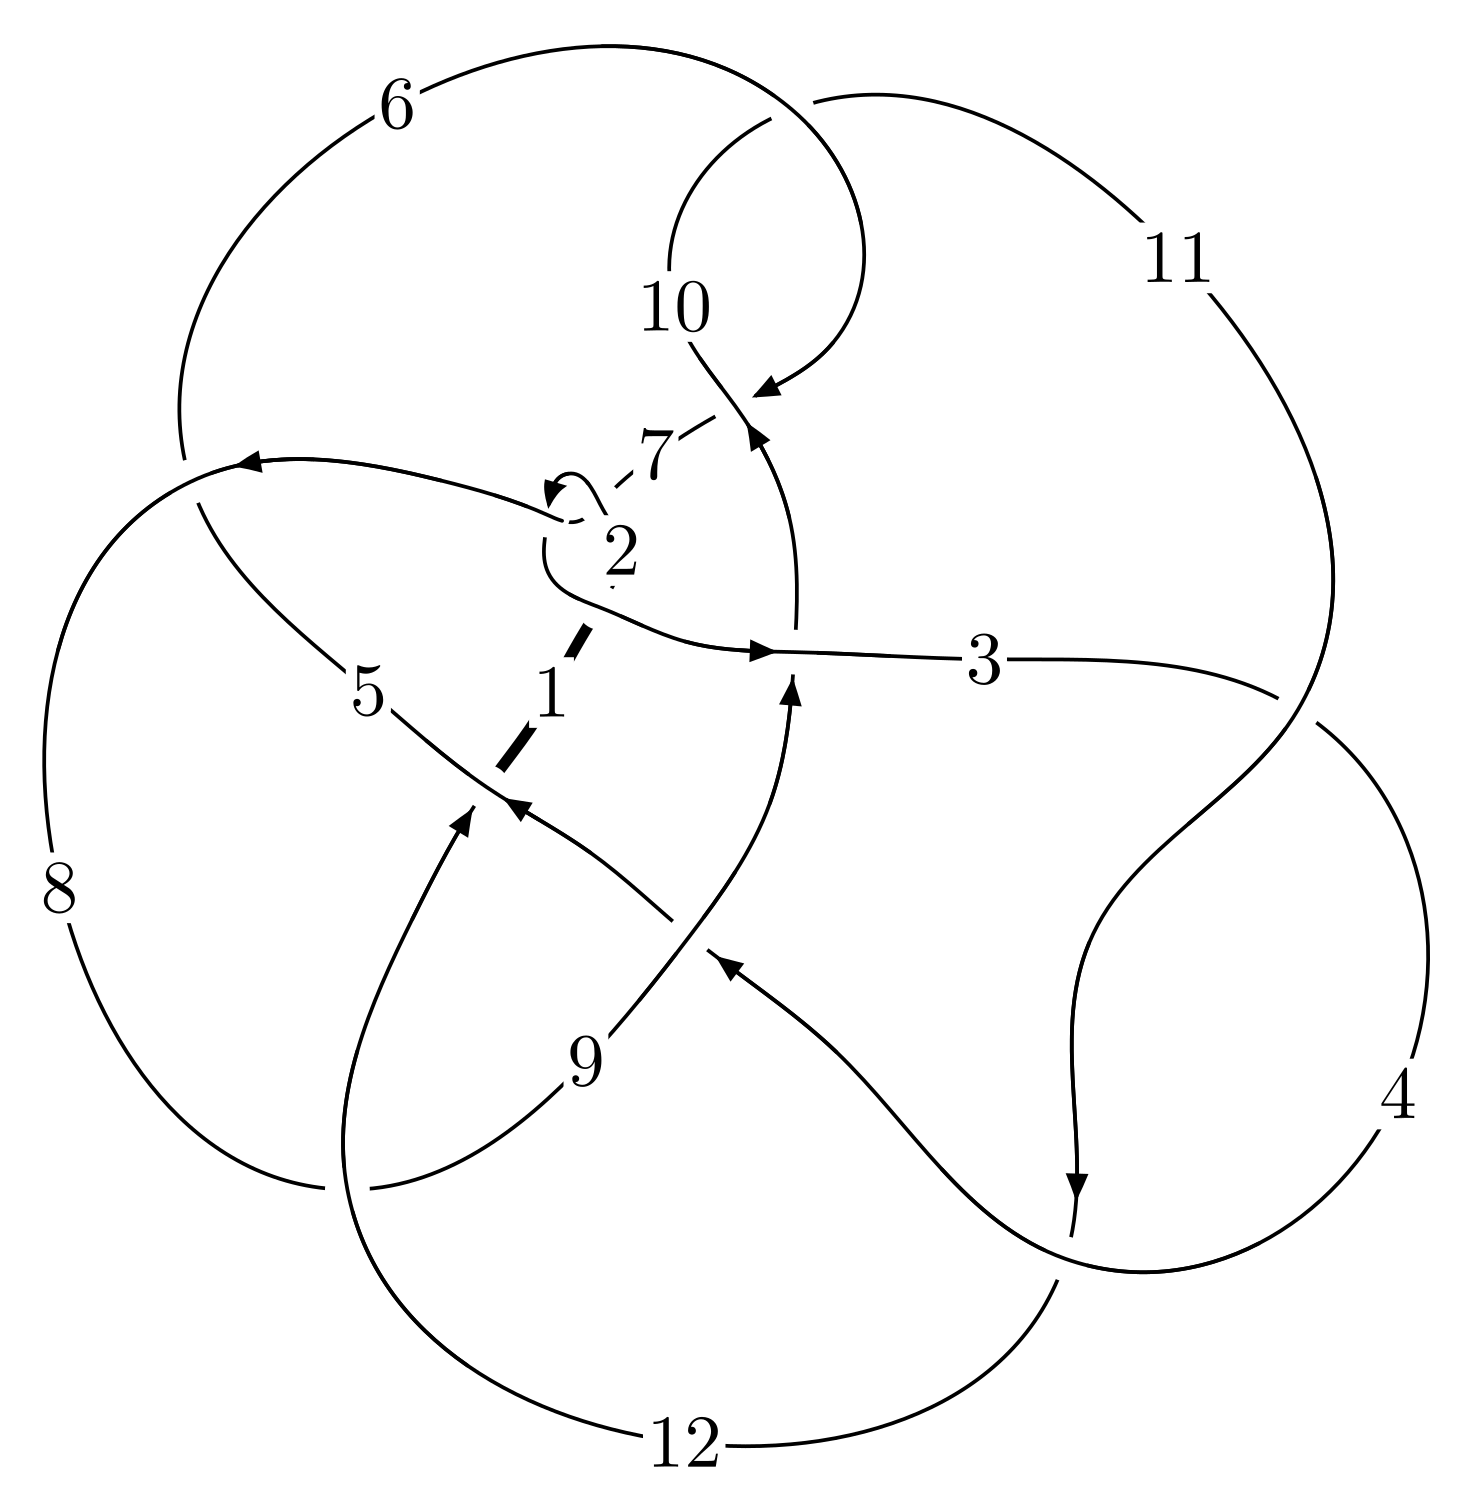
\includegraphics[width=112pt]{../../../GIT/diagram.site/Diagrams/png/2747_12n_0658.png}\\
\ \ \ A knot diagram\footnotemark}&
\allowdisplaybreaks
\textbf{Linearized knot diagam} \\
\cline{2-2}
 &
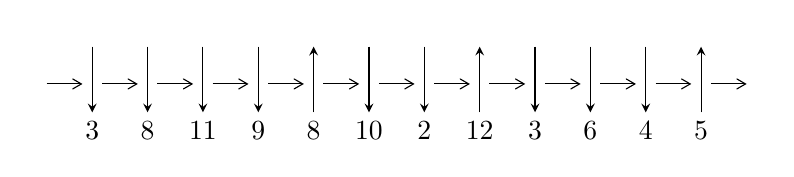
\begin{tikzpicture}[x=20pt, y=17pt]
	% nodes
	\node (C0) at (0, 0) {};
	\node (C1) at (1, 0) {};
	\node (C1U) at (1, +1) {};
	\node (C1D) at (1, -1) {3};

	\node (C2) at (2, 0) {};
	\node (C2U) at (2, +1) {};
	\node (C2D) at (2, -1) {8};

	\node (C3) at (3, 0) {};
	\node (C3U) at (3, +1) {};
	\node (C3D) at (3, -1) {11};

	\node (C4) at (4, 0) {};
	\node (C4U) at (4, +1) {};
	\node (C4D) at (4, -1) {9};

	\node (C5) at (5, 0) {};
	\node (C5U) at (5, +1) {};
	\node (C5D) at (5, -1) {8};

	\node (C6) at (6, 0) {};
	\node (C6U) at (6, +1) {};
	\node (C6D) at (6, -1) {10};

	\node (C7) at (7, 0) {};
	\node (C7U) at (7, +1) {};
	\node (C7D) at (7, -1) {2};

	\node (C8) at (8, 0) {};
	\node (C8U) at (8, +1) {};
	\node (C8D) at (8, -1) {12};

	\node (C9) at (9, 0) {};
	\node (C9U) at (9, +1) {};
	\node (C9D) at (9, -1) {3};

	\node (C10) at (10, 0) {};
	\node (C10U) at (10, +1) {};
	\node (C10D) at (10, -1) {6};

	\node (C11) at (11, 0) {};
	\node (C11U) at (11, +1) {};
	\node (C11D) at (11, -1) {4};

	\node (C12) at (12, 0) {};
	\node (C12U) at (12, +1) {};
	\node (C12D) at (12, -1) {5};
	\node (C13) at (13, 0) {};

	% arrows
	\draw[->,>={angle 60}]
	(C0) edge (C1) (C1) edge (C2) (C2) edge (C3) (C3) edge (C4) (C4) edge (C5) (C5) edge (C6) (C6) edge (C7) (C7) edge (C8) (C8) edge (C9) (C9) edge (C10) (C10) edge (C11) (C11) edge (C12) (C12) edge (C13) ;	\draw[->,>=stealth]
	(C1U) edge (C1D) (C2U) edge (C2D) (C3U) edge (C3D) (C4U) edge (C4D) (C5D) edge (C5U) (C6U) edge (C6D) (C7U) edge (C7D) (C8D) edge (C8U) (C9U) edge (C9D) (C10U) edge (C10D) (C11U) edge (C11D) (C12D) edge (C12U) ;
	\end{tikzpicture} \\
\hhline{~~} \\& 
\textbf{Solving Sequence} \\ \cline{2-2} 
 &
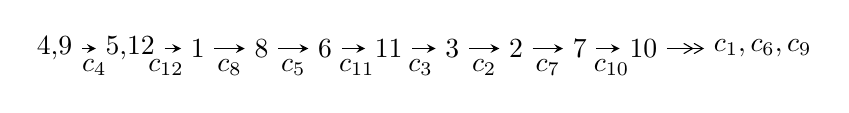
\begin{tikzpicture}[x=23pt, y=7pt]
	% node
	\node (A0) at (-1/8, 0) {4,9};
	\node (A1) at (17/16, 0) {5,12};
	\node (A2) at (17/8, 0) {1};
	\node (A3) at (25/8, 0) {8};
	\node (A4) at (33/8, 0) {6};
	\node (A5) at (41/8, 0) {11};
	\node (A6) at (49/8, 0) {3};
	\node (A7) at (57/8, 0) {2};
	\node (A8) at (65/8, 0) {7};
	\node (A9) at (73/8, 0) {10};
	\node (C1) at (1/2, -1) {$c_{4}$};
	\node (C2) at (13/8, -1) {$c_{12}$};
	\node (C3) at (21/8, -1) {$c_{8}$};
	\node (C4) at (29/8, -1) {$c_{5}$};
	\node (C5) at (37/8, -1) {$c_{11}$};
	\node (C6) at (45/8, -1) {$c_{3}$};
	\node (C7) at (53/8, -1) {$c_{2}$};
	\node (C8) at (61/8, -1) {$c_{7}$};
	\node (C9) at (69/8, -1) {$c_{10}$};
	\node (A10) at (11, 0) {$c_{1},c_{6},c_{9}$};

	% edge
	\draw[->,>=stealth]	
	(A0) edge (A1) (A1) edge (A2) (A2) edge (A3) (A3) edge (A4) (A4) edge (A5) (A5) edge (A6) (A6) edge (A7) (A7) edge (A8) (A8) edge (A9) ;
	\draw[->>,>={angle 60}]	
	(A9) edge (A10);
\end{tikzpicture} \\ 

\end{tabular} \\

\footnotetext{
The image of knot diagram is generated by the software ``\textbf{Draw programme}" developed by Andrew Bartholomew(\url{http://www.layer8.co.uk/maths/draw/index.htm\#Running-draw}), where we modified some parts for our purpose(\url{https://github.com/CATsTAILs/LinksPainter}).
}\phantom \\ \newline 
\centering \textbf{Ideals for irreducible components\footnotemark of $X_{\text{par}}$} 
 
\begin{align*}
I^u_{1}&=\langle 
1.74970\times10^{220} u^{64}-1.41335\times10^{221} u^{63}+\cdots+1.94971\times10^{223} b-7.61654\times10^{223},\\
\phantom{I^u_{1}}&\phantom{= \langle  }-4.48176\times10^{225} u^{64}-5.69453\times10^{225} u^{63}+\cdots+3.97935\times10^{226} a-1.23630\times10^{228},\\
\phantom{I^u_{1}}&\phantom{= \langle  }u^{65}+2 u^{64}+\cdots+1458 u+157\rangle \\
I^u_{2}&=\langle 
10854430144646 u^{20}+12300724825690 u^{19}+\cdots+24764957468951 b+6039231440791,\\
\phantom{I^u_{2}}&\phantom{= \langle  }-12861674233129 u^{20}-2850243387257 u^{19}+\cdots+24764957468951 a-12778119826149,\\
\phantom{I^u_{2}}&\phantom{= \langle  }u^{21}+u^{20}+\cdots-2 u^2-1\rangle \\
\\
\end{align*}
\raggedright * 2 irreducible components of $\dim_{\mathbb{C}}=0$, with total 86 representations.\\
\footnotetext{All coefficients of polynomials are rational numbers. But the coefficients are sometimes approximated in decimal forms when there is not enough margin.}
\newpage
\renewcommand{\arraystretch}{1}
\centering \section*{I. $I^u_{1}= \langle 1.75\times10^{220} u^{64}-1.41\times10^{221} u^{63}+\cdots+1.95\times10^{223} b-7.62\times10^{223},\;-4.48\times10^{225} u^{64}-5.69\times10^{225} u^{63}+\cdots+3.98\times10^{226} a-1.24\times10^{228},\;u^{65}+2 u^{64}+\cdots+1458 u+157 \rangle$}
\flushleft \textbf{(i) Arc colorings}\\
\begin{tabular}{m{7pt} m{180pt} m{7pt} m{180pt} }
\flushright $a_{4}=$&$\begin{pmatrix}1\\0\end{pmatrix}$ \\
\flushright $a_{9}=$&$\begin{pmatrix}0\\u\end{pmatrix}$ \\
\flushright $a_{5}=$&$\begin{pmatrix}1\\u^2\end{pmatrix}$ \\
\flushright $a_{12}=$&$\begin{pmatrix}0.112625 u^{64}+0.143102 u^{63}+\cdots+200.060 u+31.0678\\-0.000897414 u^{64}+0.00724903 u^{63}+\cdots+27.8175 u+3.90651\end{pmatrix}$ \\
\flushright $a_{1}=$&$\begin{pmatrix}0.0572491 u^{64}+0.0774845 u^{63}+\cdots+125.786 u+22.0769\\-0.0345792 u^{64}-0.0375444 u^{63}+\cdots-29.2953 u-3.17970\end{pmatrix}$ \\
\flushright $a_{8}=$&$\begin{pmatrix}0.173334 u^{64}+0.262177 u^{63}+\cdots+356.620 u+53.0601\\-0.0965680 u^{64}-0.124883 u^{63}+\cdots-167.497 u-21.7230\end{pmatrix}$ \\
\flushright $a_{6}=$&$\begin{pmatrix}-0.387923 u^{64}-0.492677 u^{63}+\cdots-664.492 u-77.1226\\-0.0795910 u^{64}-0.138562 u^{63}+\cdots-238.004 u-33.3801\end{pmatrix}$ \\
\flushright $a_{11}=$&$\begin{pmatrix}0.111728 u^{64}+0.150351 u^{63}+\cdots+227.877 u+34.9743\\-0.000897414 u^{64}+0.00724903 u^{63}+\cdots+27.8175 u+3.90651\end{pmatrix}$ \\
\flushright $a_{3}=$&$\begin{pmatrix}0.149474 u^{64}+0.217371 u^{63}+\cdots+298.867 u+44.4819\\0.0111114 u^{64}+0.0372127 u^{63}+\cdots+70.3743 u+10.2454\end{pmatrix}$ \\
\flushright $a_{2}=$&$\begin{pmatrix}0.154001 u^{64}+0.263124 u^{63}+\cdots+403.453 u+65.6548\\-0.165095 u^{64}-0.209683 u^{63}+\cdots-275.946 u-35.1275\end{pmatrix}$ \\
\flushright $a_{7}=$&$\begin{pmatrix}0.366877 u^{64}+0.486483 u^{63}+\cdots+650.185 u+78.1246\\0.146693 u^{64}+0.235468 u^{63}+\cdots+370.754 u+50.5795\end{pmatrix}$ \\
\flushright $a_{10}=$&$\begin{pmatrix}0.0507079 u^{64}+0.0927285 u^{63}+\cdots+147.777 u+24.8200\\-0.123127 u^{64}-0.167850 u^{63}+\cdots-230.663 u-29.1889\end{pmatrix}$\\&\end{tabular}
\flushleft \textbf{(ii) Obstruction class $= -1$}\\~\\
\flushleft \textbf{(iii) Cusp Shapes $= -0.737275 u^{64}-0.996152 u^{63}+\cdots-1391.45 u-188.248$}\\~\\
\newpage\renewcommand{\arraystretch}{1}
\flushleft \textbf{(iv) u-Polynomials at the component}\newline \\
\begin{tabular}{m{50pt}|m{274pt}}
Crossings & \hspace{64pt}u-Polynomials at each crossing \\
\hline $$\begin{aligned}c_{1}\end{aligned}$$&$\begin{aligned}
&u^{65}+80 u^{64}+\cdots+26201631 u+703921
\end{aligned}$\\
\hline $$\begin{aligned}c_{2},c_{7}\end{aligned}$$&$\begin{aligned}
&u^{65}+2 u^{64}+\cdots+2635 u-839
\end{aligned}$\\
\hline $$\begin{aligned}c_{3},c_{11}\end{aligned}$$&$\begin{aligned}
&u^{65}-25 u^{63}+\cdots-25 u-1
\end{aligned}$\\
\hline $$\begin{aligned}c_{4}\end{aligned}$$&$\begin{aligned}
&u^{65}+2 u^{64}+\cdots+1458 u+157
\end{aligned}$\\
\hline $$\begin{aligned}c_{5}\end{aligned}$$&$\begin{aligned}
&u^{65}+9 u^{64}+\cdots-13866064 u+772201
\end{aligned}$\\
\hline $$\begin{aligned}c_{6},c_{10}\end{aligned}$$&$\begin{aligned}
&u^{65}+6 u^{63}+\cdots-13 u+1
\end{aligned}$\\
\hline $$\begin{aligned}c_{8}\end{aligned}$$&$\begin{aligned}
&u^{65}+2 u^{64}+\cdots+1534 u+169
\end{aligned}$\\
\hline $$\begin{aligned}c_{9}\end{aligned}$$&$\begin{aligned}
&u^{65}+u^{64}+\cdots+626468359 u-113770343
\end{aligned}$\\
\hline $$\begin{aligned}c_{12}\end{aligned}$$&$\begin{aligned}
&u^{65}-2 u^{64}+\cdots-23392 u-2011
\end{aligned}$\\
\hline
\end{tabular}\\~\\
\newpage\renewcommand{\arraystretch}{1}
\flushleft \textbf{(v) Riley Polynomials at the component}\newline \\
\begin{tabular}{m{50pt}|m{274pt}}
Crossings & \hspace{64pt}Riley Polynomials at each crossing \\
\hline $$\begin{aligned}c_{1}\end{aligned}$$&$\begin{aligned}
&y^{65}-160 y^{64}+\cdots-124582077762381 y-495504774241
\end{aligned}$\\
\hline $$\begin{aligned}c_{2},c_{7}\end{aligned}$$&$\begin{aligned}
&y^{65}-80 y^{64}+\cdots+26201631 y-703921
\end{aligned}$\\
\hline $$\begin{aligned}c_{3},c_{11}\end{aligned}$$&$\begin{aligned}
&y^{65}-50 y^{64}+\cdots+31 y-1
\end{aligned}$\\
\hline $$\begin{aligned}c_{4}\end{aligned}$$&$\begin{aligned}
&y^{65}-14 y^{64}+\cdots+1831546 y-24649
\end{aligned}$\\
\hline $$\begin{aligned}c_{5}\end{aligned}$$&$\begin{aligned}
&y^{65}+93 y^{64}+\cdots+51698127994114 y-596294384401
\end{aligned}$\\
\hline $$\begin{aligned}c_{6},c_{10}\end{aligned}$$&$\begin{aligned}
&y^{65}+12 y^{64}+\cdots+43 y-1
\end{aligned}$\\
\hline $$\begin{aligned}c_{8}\end{aligned}$$&$\begin{aligned}
&y^{65}+16 y^{64}+\cdots-184548 y-28561
\end{aligned}$\\
\hline $$\begin{aligned}c_{9}\end{aligned}$$&$\begin{aligned}
&y^{65}-71 y^{64}+\cdots+305883945614896799 y-12943690946337649
\end{aligned}$\\
\hline $$\begin{aligned}c_{12}\end{aligned}$$&$\begin{aligned}
&y^{65}+28 y^{64}+\cdots-291747228 y-4044121
\end{aligned}$\\
\hline
\end{tabular}\\~\\
\newpage\flushleft \textbf{(vi) Complex Volumes and Cusp Shapes}
$$\begin{array}{c|c|c}  
\text{Solutions to }I^u_{1}& \I (\text{vol} + \sqrt{-1}CS) & \text{Cusp shape}\\
 \hline 
\begin{aligned}
u &= \phantom{-}0.999373 + 0.102603 I \\
a &= \phantom{-}0.183495 + 1.114360 I \\
b &= \phantom{-}1.47107 - 0.62237 I\end{aligned}
 & -13.3785 + 4.9395 I & \phantom{-0.000000 } 0 \\ \hline\begin{aligned}
u &= \phantom{-}0.999373 - 0.102603 I \\
a &= \phantom{-}0.183495 - 1.114360 I \\
b &= \phantom{-}1.47107 + 0.62237 I\end{aligned}
 & -13.3785 - 4.9395 I & \phantom{-0.000000 } 0 \\ \hline\begin{aligned}
u &= \phantom{-}0.914140 + 0.418551 I \\
a &= -0.274231 + 1.015020 I \\
b &= -0.037132 - 0.951807 I\end{aligned}
 & -0.55815 - 5.01766 I & \phantom{-0.000000 } 0 \\ \hline\begin{aligned}
u &= \phantom{-}0.914140 - 0.418551 I \\
a &= -0.274231 - 1.015020 I \\
b &= -0.037132 + 0.951807 I\end{aligned}
 & -0.55815 + 5.01766 I & \phantom{-0.000000 } 0 \\ \hline\begin{aligned}
u &= \phantom{-}0.544942 + 0.848280 I \\
a &= \phantom{-}0.017892 + 0.636408 I \\
b &= \phantom{-}0.311547 - 0.836295 I\end{aligned}
 & \phantom{-}3.81958 - 0.87527 I & \phantom{-0.000000 } 0 \\ \hline\begin{aligned}
u &= \phantom{-}0.544942 - 0.848280 I \\
a &= \phantom{-}0.017892 - 0.636408 I \\
b &= \phantom{-}0.311547 + 0.836295 I\end{aligned}
 & \phantom{-}3.81958 + 0.87527 I & \phantom{-0.000000 } 0 \\ \hline\begin{aligned}
u &= -0.943989 + 0.244778 I \\
a &= \phantom{-}1.89766 - 0.46660 I \\
b &= \phantom{-}1.322510 - 0.167180 I\end{aligned}
 & -12.02340 - 0.63123 I & \phantom{-0.000000 } 0 \\ \hline\begin{aligned}
u &= -0.943989 - 0.244778 I \\
a &= \phantom{-}1.89766 + 0.46660 I \\
b &= \phantom{-}1.322510 + 0.167180 I\end{aligned}
 & -12.02340 + 0.63123 I & \phantom{-0.000000 } 0 \\ \hline\begin{aligned}
u &= -0.718967 + 0.646460 I \\
a &= -0.19383 + 1.54085 I \\
b &= \phantom{-}1.39393 - 0.34126 I\end{aligned}
 & -3.94325 + 5.68345 I & \phantom{-0.000000 } 0 \\ \hline\begin{aligned}
u &= -0.718967 - 0.646460 I \\
a &= -0.19383 - 1.54085 I \\
b &= \phantom{-}1.39393 + 0.34126 I\end{aligned}
 & -3.94325 - 5.68345 I & \phantom{-0.000000 } 0\\
 \hline 
 \end{array}$$\newpage$$\begin{array}{c|c|c}  
\text{Solutions to }I^u_{1}& \I (\text{vol} + \sqrt{-1}CS) & \text{Cusp shape}\\
 \hline 
\begin{aligned}
u &= -0.564992 + 0.766638 I \\
a &= \phantom{-}0.273439 - 1.139240 I \\
b &= -0.098849 + 0.697594 I\end{aligned}
 & \phantom{-}0.17289 + 2.65260 I & \phantom{-0.000000 } 0 \\ \hline\begin{aligned}
u &= -0.564992 - 0.766638 I \\
a &= \phantom{-}0.273439 + 1.139240 I \\
b &= -0.098849 - 0.697594 I\end{aligned}
 & \phantom{-}0.17289 - 2.65260 I & \phantom{-0.000000 } 0 \\ \hline\begin{aligned}
u &= \phantom{-}1.032050 + 0.210054 I \\
a &= \phantom{-}0.007300 + 0.663633 I \\
b &= -1.346550 - 0.430450 I\end{aligned}
 & -4.69587 - 0.11151 I & \phantom{-0.000000 } 0 \\ \hline\begin{aligned}
u &= \phantom{-}1.032050 - 0.210054 I \\
a &= \phantom{-}0.007300 - 0.663633 I \\
b &= -1.346550 + 0.430450 I\end{aligned}
 & -4.69587 + 0.11151 I & \phantom{-0.000000 } 0 \\ \hline\begin{aligned}
u &= -1.008770 + 0.311992 I \\
a &= -0.87655 - 2.02191 I \\
b &= -1.147410 + 0.096132 I\end{aligned}
 & -3.68102 + 0.89750 I & \phantom{-0.000000 } 0 \\ \hline\begin{aligned}
u &= -1.008770 - 0.311992 I \\
a &= -0.87655 + 2.02191 I \\
b &= -1.147410 - 0.096132 I\end{aligned}
 & -3.68102 - 0.89750 I & \phantom{-0.000000 } 0 \\ \hline\begin{aligned}
u &= \phantom{-}0.819844 + 0.666051 I \\
a &= -0.04947 + 1.83615 I \\
b &= -1.264320 - 0.103822 I\end{aligned}
 & -2.80582 - 3.86569 I & \phantom{-0.000000 } 0 \\ \hline\begin{aligned}
u &= \phantom{-}0.819844 - 0.666051 I \\
a &= -0.04947 - 1.83615 I \\
b &= -1.264320 + 0.103822 I\end{aligned}
 & -2.80582 + 3.86569 I & \phantom{-0.000000 } 0 \\ \hline\begin{aligned}
u &= -1.06438\phantom{ +0.000000I} \\
a &= \phantom{-}1.18973\phantom{ +0.000000I} \\
b &= -0.491702\phantom{ +0.000000I}\end{aligned}
 & -2.53871\phantom{ +0.000000I} & \phantom{-0.000000 } 0 \\ \hline\begin{aligned}
u &= -0.861352 + 0.321812 I \\
a &= \phantom{-}0.165841 - 0.909305 I \\
b &= \phantom{-}1.47564 + 0.76252 I\end{aligned}
 & -11.72340 + 3.05933 I & -13.80482 + 0. I\phantom{ +0.000000I}\\
 \hline 
 \end{array}$$\newpage$$\begin{array}{c|c|c}  
\text{Solutions to }I^u_{1}& \I (\text{vol} + \sqrt{-1}CS) & \text{Cusp shape}\\
 \hline 
\begin{aligned}
u &= -0.861352 - 0.321812 I \\
a &= \phantom{-}0.165841 + 0.909305 I \\
b &= \phantom{-}1.47564 - 0.76252 I\end{aligned}
 & -11.72340 - 3.05933 I & -13.80482 + 0. I\phantom{ +0.000000I} \\ \hline\begin{aligned}
u &= \phantom{-}0.768490 + 0.184024 I \\
a &= \phantom{-}2.38615 + 1.30513 I \\
b &= \phantom{-}1.293180 + 0.139730 I\end{aligned}
 & -12.35970 - 6.17999 I & -13.5430 + 5.2560 I \\ \hline\begin{aligned}
u &= \phantom{-}0.768490 - 0.184024 I \\
a &= \phantom{-}2.38615 - 1.30513 I \\
b &= \phantom{-}1.293180 - 0.139730 I\end{aligned}
 & -12.35970 + 6.17999 I & -13.5430 - 5.2560 I \\ \hline\begin{aligned}
u &= \phantom{-}0.681468 + 1.023020 I \\
a &= -0.584449 - 0.266422 I \\
b &= \phantom{-}1.169520 - 0.114705 I\end{aligned}
 & -2.82139 + 3.87224 I & \phantom{-0.000000 } 0 \\ \hline\begin{aligned}
u &= \phantom{-}0.681468 - 1.023020 I \\
a &= -0.584449 + 0.266422 I \\
b &= \phantom{-}1.169520 + 0.114705 I\end{aligned}
 & -2.82139 - 3.87224 I & \phantom{-0.000000 } 0 \\ \hline\begin{aligned}
u &= \phantom{-}1.059320 + 0.651414 I \\
a &= -0.068250 - 0.898603 I \\
b &= \phantom{-}0.142000 + 1.206150 I\end{aligned}
 & -9.20705 - 1.83942 I & \phantom{-0.000000 } 0 \\ \hline\begin{aligned}
u &= \phantom{-}1.059320 - 0.651414 I \\
a &= -0.068250 + 0.898603 I \\
b &= \phantom{-}0.142000 - 1.206150 I\end{aligned}
 & -9.20705 + 1.83942 I & \phantom{-0.000000 } 0 \\ \hline\begin{aligned}
u &= -0.699109 + 0.200716 I \\
a &= \phantom{-}0.822915 - 0.817830 I \\
b &= -0.173433 + 0.242316 I\end{aligned}
 & -1.208910 + 0.548314 I & -8.64501 - 2.55655 I \\ \hline\begin{aligned}
u &= -0.699109 - 0.200716 I \\
a &= \phantom{-}0.822915 + 0.817830 I \\
b &= -0.173433 - 0.242316 I\end{aligned}
 & -1.208910 - 0.548314 I & -8.64501 + 2.55655 I \\ \hline\begin{aligned}
u &= \phantom{-}0.862620 + 1.000680 I \\
a &= -0.850831 - 0.045360 I \\
b &= -0.106228 - 0.377671 I\end{aligned}
 & -8.01748 - 4.29475 I & \phantom{-0.000000 } 0\\
 \hline 
 \end{array}$$\newpage$$\begin{array}{c|c|c}  
\text{Solutions to }I^u_{1}& \I (\text{vol} + \sqrt{-1}CS) & \text{Cusp shape}\\
 \hline 
\begin{aligned}
u &= \phantom{-}0.862620 - 1.000680 I \\
a &= -0.850831 + 0.045360 I \\
b &= -0.106228 + 0.377671 I\end{aligned}
 & -8.01748 + 4.29475 I & \phantom{-0.000000 } 0 \\ \hline\begin{aligned}
u &= \phantom{-}1.158140 + 0.659100 I \\
a &= \phantom{-}0.117313 - 1.313300 I \\
b &= \phantom{-}1.318680 + 0.427978 I\end{aligned}
 & -4.81417 - 9.90537 I & \phantom{-0.000000 } 0 \\ \hline\begin{aligned}
u &= \phantom{-}1.158140 - 0.659100 I \\
a &= \phantom{-}0.117313 + 1.313300 I \\
b &= \phantom{-}1.318680 - 0.427978 I\end{aligned}
 & -4.81417 + 9.90537 I & \phantom{-0.000000 } 0 \\ \hline\begin{aligned}
u &= \phantom{-}0.512850 + 0.407512 I \\
a &= -0.54396 + 1.92014 I \\
b &= -1.227830 - 0.206235 I\end{aligned}
 & -1.82076 - 0.96957 I & -1.84094 - 0.74780 I \\ \hline\begin{aligned}
u &= \phantom{-}0.512850 - 0.407512 I \\
a &= -0.54396 - 1.92014 I \\
b &= -1.227830 + 0.206235 I\end{aligned}
 & -1.82076 + 0.96957 I & -1.84094 + 0.74780 I \\ \hline\begin{aligned}
u &= -1.075290 + 0.820321 I \\
a &= \phantom{-}0.029326 + 0.907628 I \\
b &= \phantom{-}0.210489 - 1.168250 I\end{aligned}
 & -8.16440 + 10.11900 I & \phantom{-0.000000 } 0 \\ \hline\begin{aligned}
u &= -1.075290 - 0.820321 I \\
a &= \phantom{-}0.029326 - 0.907628 I \\
b &= \phantom{-}0.210489 + 1.168250 I\end{aligned}
 & -8.16440 - 10.11900 I & \phantom{-0.000000 } 0 \\ \hline\begin{aligned}
u &= -0.633443 + 0.121495 I \\
a &= \phantom{-}0.80489 - 1.99874 I \\
b &= -1.072970 + 0.269722 I\end{aligned}
 & -2.58233 + 0.73416 I & -9.39358 + 8.45936 I \\ \hline\begin{aligned}
u &= -0.633443 - 0.121495 I \\
a &= \phantom{-}0.80489 + 1.99874 I \\
b &= -1.072970 - 0.269722 I\end{aligned}
 & -2.58233 - 0.73416 I & -9.39358 - 8.45936 I \\ \hline\begin{aligned}
u &= -1.144370 + 0.749445 I \\
a &= \phantom{-}0.001986 - 0.627491 I \\
b &= -1.32660 + 0.55872 I\end{aligned}
 & -1.63568 + 5.32861 I & \phantom{-0.000000 } 0\\
 \hline 
 \end{array}$$\newpage$$\begin{array}{c|c|c}  
\text{Solutions to }I^u_{1}& \I (\text{vol} + \sqrt{-1}CS) & \text{Cusp shape}\\
 \hline 
\begin{aligned}
u &= -1.144370 - 0.749445 I \\
a &= \phantom{-}0.001986 + 0.627491 I \\
b &= -1.32660 - 0.55872 I\end{aligned}
 & -1.63568 - 5.32861 I & \phantom{-0.000000 } 0 \\ \hline\begin{aligned}
u &= \phantom{-}0.551203 + 0.205508 I \\
a &= \phantom{-}0.96007 - 1.78056 I \\
b &= -0.0840652 + 0.0654924 I\end{aligned}
 & \phantom{-}0.93353 - 2.84266 I & -8.27444 - 0.53942 I \\ \hline\begin{aligned}
u &= \phantom{-}0.551203 - 0.205508 I \\
a &= \phantom{-}0.96007 + 1.78056 I \\
b &= -0.0840652 - 0.0654924 I\end{aligned}
 & \phantom{-}0.93353 + 2.84266 I & -8.27444 + 0.53942 I \\ \hline\begin{aligned}
u &= -0.94708 + 1.13082 I \\
a &= -0.289084 + 0.976259 I \\
b &= \phantom{-}1.321940 - 0.311580 I\end{aligned}
 & -4.26583 + 6.35751 I & \phantom{-0.000000 } 0 \\ \hline\begin{aligned}
u &= -0.94708 - 1.13082 I \\
a &= -0.289084 - 0.976259 I \\
b &= \phantom{-}1.321940 + 0.311580 I\end{aligned}
 & -4.26583 - 6.35751 I & \phantom{-0.000000 } 0 \\ \hline\begin{aligned}
u &= -0.96950 + 1.11387 I \\
a &= -0.666748 - 0.221312 I \\
b &= -0.152577 + 0.535195 I\end{aligned}
 & -7.36307 - 3.09669 I & \phantom{-0.000000 } 0 \\ \hline\begin{aligned}
u &= -0.96950 - 1.11387 I \\
a &= -0.666748 + 0.221312 I \\
b &= -0.152577 - 0.535195 I\end{aligned}
 & -7.36307 + 3.09669 I & \phantom{-0.000000 } 0 \\ \hline\begin{aligned}
u &= \phantom{-}0.017003 + 0.520994 I \\
a &= \phantom{-}0.52264 - 1.79134 I \\
b &= -0.170066 + 0.616830 I\end{aligned}
 & \phantom{-}1.35247 + 2.01752 I & -0.32815 - 3.57932 I \\ \hline\begin{aligned}
u &= \phantom{-}0.017003 - 0.520994 I \\
a &= \phantom{-}0.52264 + 1.79134 I \\
b &= -0.170066 - 0.616830 I\end{aligned}
 & \phantom{-}1.35247 - 2.01752 I & -0.32815 + 3.57932 I \\ \hline\begin{aligned}
u &= -0.487051 + 0.184553 I \\
a &= -0.523976 + 0.683896 I \\
b &= -0.364029 - 1.277030 I\end{aligned}
 & \phantom{-}2.05730 - 1.12785 I & -14.5677 + 6.0985 I\\
 \hline 
 \end{array}$$\newpage$$\begin{array}{c|c|c}  
\text{Solutions to }I^u_{1}& \I (\text{vol} + \sqrt{-1}CS) & \text{Cusp shape}\\
 \hline 
\begin{aligned}
u &= -0.487051 - 0.184553 I \\
a &= -0.523976 - 0.683896 I \\
b &= -0.364029 + 1.277030 I\end{aligned}
 & \phantom{-}2.05730 + 1.12785 I & -14.5677 - 6.0985 I \\ \hline\begin{aligned}
u &= \phantom{-}1.34403 + 0.87395 I \\
a &= \phantom{-}0.245632 - 0.677061 I \\
b &= \phantom{-}1.137180 + 0.382997 I\end{aligned}
 & \phantom{-}1.20608 - 5.29372 I & \phantom{-0.000000 } 0 \\ \hline\begin{aligned}
u &= \phantom{-}1.34403 - 0.87395 I \\
a &= \phantom{-}0.245632 + 0.677061 I \\
b &= \phantom{-}1.137180 - 0.382997 I\end{aligned}
 & \phantom{-}1.20608 + 5.29372 I & \phantom{-0.000000 } 0 \\ \hline\begin{aligned}
u &= -1.62477\phantom{ +0.000000I} \\
a &= \phantom{-}0.128143\phantom{ +0.000000I} \\
b &= \phantom{-}1.37061\phantom{ +0.000000I}\end{aligned}
 & -8.24749\phantom{ +0.000000I} & \phantom{-0.000000 } 0 \\ \hline\begin{aligned}
u &= \phantom{-}1.48370 + 0.87202 I \\
a &= -0.057752 + 0.890430 I \\
b &= -1.44306 - 0.50190 I\end{aligned}
 & -14.2637 - 7.7830 I & \phantom{-0.000000 } 0 \\ \hline\begin{aligned}
u &= \phantom{-}1.48370 - 0.87202 I \\
a &= -0.057752 - 0.890430 I \\
b &= -1.44306 + 0.50190 I\end{aligned}
 & -14.2637 + 7.7830 I & \phantom{-0.000000 } 0 \\ \hline\begin{aligned}
u &= -1.44711 + 0.93929 I \\
a &= -0.099582 - 0.974443 I \\
b &= -1.45292 + 0.48475 I\end{aligned}
 & -13.4195 + 15.8987 I & \phantom{-0.000000 } 0 \\ \hline\begin{aligned}
u &= -1.44711 - 0.93929 I \\
a &= -0.099582 + 0.974443 I \\
b &= -1.45292 - 0.48475 I\end{aligned}
 & -13.4195 - 15.8987 I & \phantom{-0.000000 } 0 \\ \hline\begin{aligned}
u &= -1.37855 + 1.03960 I \\
a &= -0.123840 + 0.435880 I \\
b &= \phantom{-}1.190040 - 0.087701 I\end{aligned}
 & -4.94093 + 1.63213 I & \phantom{-0.000000 } 0 \\ \hline\begin{aligned}
u &= -1.37855 - 1.03960 I \\
a &= -0.123840 - 0.435880 I \\
b &= \phantom{-}1.190040 + 0.087701 I\end{aligned}
 & -4.94093 - 1.63213 I & \phantom{-0.000000 } 0\\
 \hline 
 \end{array}$$\newpage$$\begin{array}{c|c|c}  
\text{Solutions to }I^u_{1}& \I (\text{vol} + \sqrt{-1}CS) & \text{Cusp shape}\\
 \hline 
\begin{aligned}
u &= -0.144278\phantom{ +0.000000I} \\
a &= \phantom{-}5.40384\phantom{ +0.000000I} \\
b &= -0.674268\phantom{ +0.000000I}\end{aligned}
 & -1.17407\phantom{ +0.000000I} & -8.98220\phantom{ +0.000000I} \\ \hline\begin{aligned}
u &= \phantom{-}1.62504 + 2.08961 I \\
a &= \phantom{-}0.195235 + 0.198274 I \\
b &= -1.214090 + 0.100227 I\end{aligned}
 & -11.29140 - 2.66062 I & \phantom{-0.000000 } 0 \\ \hline\begin{aligned}
u &= \phantom{-}1.62504 - 2.08961 I \\
a &= \phantom{-}0.195235 - 0.198274 I \\
b &= -1.214090 - 0.100227 I\end{aligned}
 & -11.29140 + 2.66062 I & \phantom{-0.000000 } 0 \\ \hline\begin{aligned}
u &= -1.07793 + 2.55737 I \\
a &= \phantom{-}0.184452 + 0.002607 I \\
b &= -1.177930 - 0.198966 I\end{aligned}
 & -10.35930 - 5.79368 I & \phantom{-0.000000 } 0 \\ \hline\begin{aligned}
u &= -1.07793 - 2.55737 I \\
a &= \phantom{-}0.184452 - 0.002607 I \\
b &= -1.177930 + 0.198966 I\end{aligned}
 & -10.35930 + 5.79368 I & \phantom{-0.000000 } 0\\
 \hline 
 \end{array}$$\newpage\newpage\renewcommand{\arraystretch}{1}
\centering \section*{II. $I^u_{2}= \langle 1.09\times10^{13} u^{20}+1.23\times10^{13} u^{19}+\cdots+2.48\times10^{13} b+6.04\times10^{12},\;-1.29\times10^{13} u^{20}-2.85\times10^{12} u^{19}+\cdots+2.48\times10^{13} a-1.28\times10^{13},\;u^{21}+u^{20}+\cdots-2 u^2-1 \rangle$}
\flushleft \textbf{(i) Arc colorings}\\
\begin{tabular}{m{7pt} m{180pt} m{7pt} m{180pt} }
\flushright $a_{4}=$&$\begin{pmatrix}1\\0\end{pmatrix}$ \\
\flushright $a_{9}=$&$\begin{pmatrix}0\\u\end{pmatrix}$ \\
\flushright $a_{5}=$&$\begin{pmatrix}1\\u^2\end{pmatrix}$ \\
\flushright $a_{12}=$&$\begin{pmatrix}0.519350 u^{20}+0.115092 u^{19}+\cdots+4.75906 u+0.515976\\-0.438298 u^{20}-0.496699 u^{19}+\cdots-1.49110 u-0.243862\end{pmatrix}$ \\
\flushright $a_{1}=$&$\begin{pmatrix}0.432185 u^{20}-0.347015 u^{19}+\cdots+2.74861 u+0.676372\\0.0360697 u^{20}-0.276002 u^{19}+\cdots-1.57826 u-0.618804\end{pmatrix}$ \\
\flushright $a_{8}=$&$\begin{pmatrix}0.343067 u^{20}+0.800587 u^{19}+\cdots+0.543328 u+2.17015\\-0.349292 u^{20}-0.630439 u^{19}+\cdots+2.20499 u+0.0265777\end{pmatrix}$ \\
\flushright $a_{6}=$&$\begin{pmatrix}0.561265 u^{20}+1.60373 u^{19}+\cdots-5.73182 u-0.208417\\0.0890616 u^{20}-0.213890 u^{19}+\cdots+2.41615 u+1.51061\end{pmatrix}$ \\
\flushright $a_{11}=$&$\begin{pmatrix}0.0810518 u^{20}-0.381607 u^{19}+\cdots+3.26796 u+0.272114\\-0.438298 u^{20}-0.496699 u^{19}+\cdots-1.49110 u-0.243862\end{pmatrix}$ \\
\flushright $a_{3}=$&$\begin{pmatrix}-0.713332 u^{20}-0.888724 u^{19}+\cdots+4.27797 u+1.97434\\-0.739910 u^{20}-0.566010 u^{19}+\cdots-2.10462 u-0.230652\end{pmatrix}$ \\
\flushright $a_{2}=$&$\begin{pmatrix}0.0219095 u^{20}-0.283308 u^{19}+\cdots+2.48653 u+0.812160\\-0.519367 u^{20}-0.445460 u^{19}+\cdots-2.03367 u+0.145816\end{pmatrix}$ \\
\flushright $a_{7}=$&$\begin{pmatrix}1.01832 u^{20}+1.08146 u^{19}+\cdots+1.09672 u+1.27496\\0.272340 u^{20}-0.310322 u^{19}+\cdots+2.54320 u-0.924913\end{pmatrix}$ \\
\flushright $a_{10}=$&$\begin{pmatrix}0.684289 u^{20}+0.403574 u^{19}+\cdots+1.29439 u+3.50062\\-0.623557 u^{20}-1.06224 u^{19}+\cdots+1.98393 u-0.232468\end{pmatrix}$\\&\end{tabular}
\flushleft \textbf{(ii) Obstruction class $= 1$}\\~\\
\flushleft \textbf{(iii) Cusp Shapes $= \frac{11118351519795}{24764957468951} u^{20}-\frac{6479749559907}{3537851066993} u^{19}+\cdots-\frac{134928284668245}{24764957468951} u-\frac{205361301351383}{24764957468951}$}\\~\\
\newpage\renewcommand{\arraystretch}{1}
\flushleft \textbf{(iv) u-Polynomials at the component}\newline \\
\begin{tabular}{m{50pt}|m{274pt}}
Crossings & \hspace{64pt}u-Polynomials at each crossing \\
\hline $$\begin{aligned}c_{1}\end{aligned}$$&$\begin{aligned}
&u^{21}-21 u^{20}+\cdots-3 u-1
\end{aligned}$\\
\hline $$\begin{aligned}c_{2}\end{aligned}$$&$\begin{aligned}
&u^{21}- u^{20}+\cdots+3 u-1
\end{aligned}$\\
\hline $$\begin{aligned}c_{3}\end{aligned}$$&$\begin{aligned}
&u^{21}- u^{20}+\cdots+11 u+7
\end{aligned}$\\
\hline $$\begin{aligned}c_{4}\end{aligned}$$&$\begin{aligned}
&u^{21}+u^{20}+\cdots-2 u^2-1
\end{aligned}$\\
\hline $$\begin{aligned}c_{5}\end{aligned}$$&$\begin{aligned}
&u^{21}+2 u^{20}+\cdots+6 u-7
\end{aligned}$\\
\hline $$\begin{aligned}c_{6}\end{aligned}$$&$\begin{aligned}
&u^{21}+u^{20}+\cdots- u+1
\end{aligned}$\\
\hline $$\begin{aligned}c_{7}\end{aligned}$$&$\begin{aligned}
&u^{21}+u^{20}+\cdots+3 u+1
\end{aligned}$\\
\hline $$\begin{aligned}c_{8}\end{aligned}$$&$\begin{aligned}
&u^{21}+u^{20}+\cdots-4 u+1
\end{aligned}$\\
\hline $$\begin{aligned}c_{9}\end{aligned}$$&$\begin{aligned}
&u^{21}+2 u^{20}+\cdots-71 u+19
\end{aligned}$\\
\hline $$\begin{aligned}c_{10}\end{aligned}$$&$\begin{aligned}
&u^{21}- u^{20}+\cdots- u-1
\end{aligned}$\\
\hline $$\begin{aligned}c_{11}\end{aligned}$$&$\begin{aligned}
&u^{21}+u^{20}+\cdots+11 u-7
\end{aligned}$\\
\hline $$\begin{aligned}c_{12}\end{aligned}$$&$\begin{aligned}
&u^{21}-3 u^{20}+\cdots+2 u-1
\end{aligned}$\\
\hline
\end{tabular}\\~\\
\newpage\renewcommand{\arraystretch}{1}
\flushleft \textbf{(v) Riley Polynomials at the component}\newline \\
\begin{tabular}{m{50pt}|m{274pt}}
Crossings & \hspace{64pt}Riley Polynomials at each crossing \\
\hline $$\begin{aligned}c_{1}\end{aligned}$$&$\begin{aligned}
&y^{21}-53 y^{20}+\cdots+73 y-1
\end{aligned}$\\
\hline $$\begin{aligned}c_{2},c_{7}\end{aligned}$$&$\begin{aligned}
&y^{21}-21 y^{20}+\cdots-3 y-1
\end{aligned}$\\
\hline $$\begin{aligned}c_{3},c_{11}\end{aligned}$$&$\begin{aligned}
&y^{21}-15 y^{20}+\cdots+93 y-49
\end{aligned}$\\
\hline $$\begin{aligned}c_{4}\end{aligned}$$&$\begin{aligned}
&y^{21}+5 y^{20}+\cdots-4 y-1
\end{aligned}$\\
\hline $$\begin{aligned}c_{5}\end{aligned}$$&$\begin{aligned}
&y^{21}-12 y^{20}+\cdots+2108 y-49
\end{aligned}$\\
\hline $$\begin{aligned}c_{6},c_{10}\end{aligned}$$&$\begin{aligned}
&y^{21}+15 y^{20}+\cdots+5 y-1
\end{aligned}$\\
\hline $$\begin{aligned}c_{8}\end{aligned}$$&$\begin{aligned}
&y^{21}+3 y^{20}+\cdots+6 y-1
\end{aligned}$\\
\hline $$\begin{aligned}c_{9}\end{aligned}$$&$\begin{aligned}
&y^{21}-8 y^{20}+\cdots-6815 y-361
\end{aligned}$\\
\hline $$\begin{aligned}c_{12}\end{aligned}$$&$\begin{aligned}
&y^{21}- y^{20}+\cdots+2 y-1
\end{aligned}$\\
\hline
\end{tabular}\\~\\
\newpage\flushleft \textbf{(vi) Complex Volumes and Cusp Shapes}
$$\begin{array}{c|c|c}  
\text{Solutions to }I^u_{2}& \I (\text{vol} + \sqrt{-1}CS) & \text{Cusp shape}\\
 \hline 
\begin{aligned}
u &= \phantom{-}0.995040\phantom{ +0.000000I} \\
a &= \phantom{-}1.53732\phantom{ +0.000000I} \\
b &= -0.633509\phantom{ +0.000000I}\end{aligned}
 & -2.63990\phantom{ +0.000000I} & -61.2880\phantom{ +0.000000I} \\ \hline\begin{aligned}
u &= \phantom{-}0.887942 + 0.265832 I \\
a &= -0.27186 + 1.60857 I \\
b &= -1.105880 - 0.231970 I\end{aligned}
 & -3.10576 - 1.08145 I & -11.60473 - 1.20772 I \\ \hline\begin{aligned}
u &= \phantom{-}0.887942 - 0.265832 I \\
a &= -0.27186 - 1.60857 I \\
b &= -1.105880 + 0.231970 I\end{aligned}
 & -3.10576 + 1.08145 I & -11.60473 + 1.20772 I \\ \hline\begin{aligned}
u &= \phantom{-}0.335007 + 0.764873 I \\
a &= \phantom{-}0.349475 + 0.797361 I \\
b &= \phantom{-}0.126425 - 1.048160 I\end{aligned}
 & \phantom{-}2.99868 - 1.45719 I & -4.59366 + 6.14585 I \\ \hline\begin{aligned}
u &= \phantom{-}0.335007 - 0.764873 I \\
a &= \phantom{-}0.349475 - 0.797361 I \\
b &= \phantom{-}0.126425 + 1.048160 I\end{aligned}
 & \phantom{-}2.99868 + 1.45719 I & -4.59366 - 6.14585 I \\ \hline\begin{aligned}
u &= -0.768678 + 0.960873 I \\
a &= -0.391291 + 1.331950 I \\
b &= \phantom{-}1.355210 - 0.281637 I\end{aligned}
 & -3.38645 + 6.55264 I & -3.36004 - 8.68236 I \\ \hline\begin{aligned}
u &= -0.768678 - 0.960873 I \\
a &= -0.391291 - 1.331950 I \\
b &= \phantom{-}1.355210 + 0.281637 I\end{aligned}
 & -3.38645 - 6.55264 I & -3.36004 + 8.68236 I \\ \hline\begin{aligned}
u &= -0.480430 + 0.542921 I \\
a &= \phantom{-}0.03174 - 1.74407 I \\
b &= -0.102734 + 0.532504 I\end{aligned}
 & \phantom{-}1.33027 + 3.34421 I & \phantom{-}0.81047 - 9.50324 I \\ \hline\begin{aligned}
u &= -0.480430 - 0.542921 I \\
a &= \phantom{-}0.03174 + 1.74407 I \\
b &= -0.102734 - 0.532504 I\end{aligned}
 & \phantom{-}1.33027 - 3.34421 I & \phantom{-}0.81047 + 9.50324 I \\ \hline\begin{aligned}
u &= -0.598889 + 0.406001 I \\
a &= \phantom{-}0.173713 + 0.637671 I \\
b &= -0.631828 - 1.130440 I\end{aligned}
 & \phantom{-}2.34945 - 0.74831 I & -4.02686 - 6.25327 I\\
 \hline 
 \end{array}$$\newpage$$\begin{array}{c|c|c}  
\text{Solutions to }I^u_{2}& \I (\text{vol} + \sqrt{-1}CS) & \text{Cusp shape}\\
 \hline 
\begin{aligned}
u &= -0.598889 - 0.406001 I \\
a &= \phantom{-}0.173713 - 0.637671 I \\
b &= -0.631828 + 1.130440 I\end{aligned}
 & \phantom{-}2.34945 + 0.74831 I & -4.02686 + 6.25327 I \\ \hline\begin{aligned}
u &= -1.166620 + 0.527651 I \\
a &= -0.579151 - 0.728388 I \\
b &= -1.089360 + 0.405520 I\end{aligned}
 & \phantom{-}0.49818 + 4.56432 I & -8.19695 - 3.48083 I \\ \hline\begin{aligned}
u &= -1.166620 - 0.527651 I \\
a &= -0.579151 + 0.728388 I \\
b &= -1.089360 - 0.405520 I\end{aligned}
 & \phantom{-}0.49818 - 4.56432 I & -8.19695 + 3.48083 I \\ \hline\begin{aligned}
u &= -0.725758 + 1.061050 I \\
a &= \phantom{-}0.271335 + 0.349520 I \\
b &= \phantom{-}1.175310 + 0.315124 I\end{aligned}
 & -10.06770 + 2.53564 I & -8.77876 - 1.65013 I \\ \hline\begin{aligned}
u &= -0.725758 - 1.061050 I \\
a &= \phantom{-}0.271335 - 0.349520 I \\
b &= \phantom{-}1.175310 - 0.315124 I\end{aligned}
 & -10.06770 - 2.53564 I & -8.77876 + 1.65013 I \\ \hline\begin{aligned}
u &= \phantom{-}0.216516 + 0.360136 I \\
a &= \phantom{-}2.00760 + 2.33089 I \\
b &= -1.304550 - 0.087060 I\end{aligned}
 & -3.10125 - 2.22500 I & -10.50218 + 2.63419 I \\ \hline\begin{aligned}
u &= \phantom{-}0.216516 - 0.360136 I \\
a &= \phantom{-}2.00760 - 2.33089 I \\
b &= -1.304550 + 0.087060 I\end{aligned}
 & -3.10125 + 2.22500 I & -10.50218 - 2.63419 I \\ \hline\begin{aligned}
u &= \phantom{-}1.06547 + 1.24110 I \\
a &= -0.085748 - 0.678299 I \\
b &= \phantom{-}1.279400 + 0.468268 I\end{aligned}
 & -0.73617 - 6.70838 I & -6.14219 + 7.52338 I \\ \hline\begin{aligned}
u &= \phantom{-}1.06547 - 1.24110 I \\
a &= -0.085748 + 0.678299 I \\
b &= \phantom{-}1.279400 - 0.468268 I\end{aligned}
 & -0.73617 + 6.70838 I & -6.14219 - 7.52338 I \\ \hline\begin{aligned}
u &= \phantom{-}0.23792 + 1.75774 I \\
a &= -0.274467 - 0.304190 I \\
b &= \phantom{-}1.114760 - 0.227134 I\end{aligned}
 & -10.13330 + 5.08046 I & -10.46087 - 0.93338 I\\
 \hline 
 \end{array}$$\newpage$$\begin{array}{c|c|c}  
\text{Solutions to }I^u_{2}& \I (\text{vol} + \sqrt{-1}CS) & \text{Cusp shape}\\
 \hline 
\begin{aligned}
u &= \phantom{-}0.23792 - 1.75774 I \\
a &= -0.274467 + 0.304190 I \\
b &= \phantom{-}1.114760 + 0.227134 I\end{aligned}
 & -10.13330 - 5.08046 I & -10.46087 + 0.93338 I\\
 \hline 
 \end{array}$$\newpage
\newpage\renewcommand{\arraystretch}{1}
\centering \section*{ III. u-Polynomials}
\begin{tabular}{m{50pt}|m{274pt}}
Crossings & \hspace{64pt}u-Polynomials at each crossing \\
\hline $$\begin{aligned}c_{1}\end{aligned}$$&$\begin{aligned}
&(u^{21}-21 u^{20}+\cdots-3 u-1)\\
&\cdot(u^{65}+80 u^{64}+\cdots+26201631 u+703921)
\end{aligned}$\\
\hline $$\begin{aligned}c_{2}\end{aligned}$$&$\begin{aligned}
&(u^{21}- u^{20}+\cdots+3 u-1)(u^{65}+2 u^{64}+\cdots+2635 u-839)
\end{aligned}$\\
\hline $$\begin{aligned}c_{3}\end{aligned}$$&$\begin{aligned}
&(u^{21}- u^{20}+\cdots+11 u+7)(u^{65}-25 u^{63}+\cdots-25 u-1)
\end{aligned}$\\
\hline $$\begin{aligned}c_{4}\end{aligned}$$&$\begin{aligned}
&(u^{21}+u^{20}+\cdots-2 u^2-1)(u^{65}+2 u^{64}+\cdots+1458 u+157)
\end{aligned}$\\
\hline $$\begin{aligned}c_{5}\end{aligned}$$&$\begin{aligned}
&(u^{21}+2 u^{20}+\cdots+6 u-7)(u^{65}+9 u^{64}+\cdots-1.38661\times10^{7} u+772201)
\end{aligned}$\\
\hline $$\begin{aligned}c_{6}\end{aligned}$$&$\begin{aligned}
&(u^{21}+u^{20}+\cdots- u+1)(u^{65}+6 u^{63}+\cdots-13 u+1)
\end{aligned}$\\
\hline $$\begin{aligned}c_{7}\end{aligned}$$&$\begin{aligned}
&(u^{21}+u^{20}+\cdots+3 u+1)(u^{65}+2 u^{64}+\cdots+2635 u-839)
\end{aligned}$\\
\hline $$\begin{aligned}c_{8}\end{aligned}$$&$\begin{aligned}
&(u^{21}+u^{20}+\cdots-4 u+1)(u^{65}+2 u^{64}+\cdots+1534 u+169)
\end{aligned}$\\
\hline $$\begin{aligned}c_{9}\end{aligned}$$&$\begin{aligned}
&(u^{21}+2 u^{20}+\cdots-71 u+19)\\
&\cdot(u^{65}+u^{64}+\cdots+626468359 u-113770343)
\end{aligned}$\\
\hline $$\begin{aligned}c_{10}\end{aligned}$$&$\begin{aligned}
&(u^{21}- u^{20}+\cdots- u-1)(u^{65}+6 u^{63}+\cdots-13 u+1)
\end{aligned}$\\
\hline $$\begin{aligned}c_{11}\end{aligned}$$&$\begin{aligned}
&(u^{21}+u^{20}+\cdots+11 u-7)(u^{65}-25 u^{63}+\cdots-25 u-1)
\end{aligned}$\\
\hline $$\begin{aligned}c_{12}\end{aligned}$$&$\begin{aligned}
&(u^{21}-3 u^{20}+\cdots+2 u-1)(u^{65}-2 u^{64}+\cdots-23392 u-2011)
\end{aligned}$\\
\hline
\end{tabular}\newpage\renewcommand{\arraystretch}{1}
\centering \section*{ IV. Riley Polynomials}
\begin{tabular}{m{50pt}|m{274pt}}
Crossings & \hspace{64pt}Riley Polynomials at each crossing \\
\hline $$\begin{aligned}c_{1}\end{aligned}$$&$\begin{aligned}
&(y^{21}-53 y^{20}+\cdots+73 y-1)\\
&\cdot(y^{65}-160 y^{64}+\cdots-124582077762381 y-495504774241)
\end{aligned}$\\
\hline $$\begin{aligned}c_{2},c_{7}\end{aligned}$$&$\begin{aligned}
&(y^{21}-21 y^{20}+\cdots-3 y-1)\\
&\cdot(y^{65}-80 y^{64}+\cdots+26201631 y-703921)
\end{aligned}$\\
\hline $$\begin{aligned}c_{3},c_{11}\end{aligned}$$&$\begin{aligned}
&(y^{21}-15 y^{20}+\cdots+93 y-49)(y^{65}-50 y^{64}+\cdots+31 y-1)
\end{aligned}$\\
\hline $$\begin{aligned}c_{4}\end{aligned}$$&$\begin{aligned}
&(y^{21}+5 y^{20}+\cdots-4 y-1)(y^{65}-14 y^{64}+\cdots+1831546 y-24649)
\end{aligned}$\\
\hline $$\begin{aligned}c_{5}\end{aligned}$$&$\begin{aligned}
&(y^{21}-12 y^{20}+\cdots+2108 y-49)\\
&\cdot(y^{65}+93 y^{64}+\cdots+51698127994114 y-596294384401)
\end{aligned}$\\
\hline $$\begin{aligned}c_{6},c_{10}\end{aligned}$$&$\begin{aligned}
&(y^{21}+15 y^{20}+\cdots+5 y-1)(y^{65}+12 y^{64}+\cdots+43 y-1)
\end{aligned}$\\
\hline $$\begin{aligned}c_{8}\end{aligned}$$&$\begin{aligned}
&(y^{21}+3 y^{20}+\cdots+6 y-1)(y^{65}+16 y^{64}+\cdots-184548 y-28561)
\end{aligned}$\\
\hline $$\begin{aligned}c_{9}\end{aligned}$$&$\begin{aligned}
&(y^{21}-8 y^{20}+\cdots-6815 y-361)\\
&\cdot(y^{65}-71 y^{64}+\cdots+305883945614896799 y-12943690946337649)
\end{aligned}$\\
\hline $$\begin{aligned}c_{12}\end{aligned}$$&$\begin{aligned}
&(y^{21}- y^{20}+\cdots+2 y-1)\\
&\cdot(y^{65}+28 y^{64}+\cdots-291747228 y-4044121)
\end{aligned}$\\
\hline
\end{tabular}
\vskip 2pc
\end{document}